\documentclass{article} % For LaTeX2e
\usepackage{xr}
%\externaldocument{Appendix}


\usepackage{nips15submit_e,times}



%=========================================================
% Standard Packages
%=========================================================

\usepackage[numbers]{natbib}
\usepackage{hyperref}
\usepackage{url}
\usepackage{amsmath,amsthm,amsfonts,amssymb,mathtools, fancyvrb}
\usepackage{algorithm,algorithmic}
%\usepackage[noend]{,amssymb,amsfonts,amsmath}
%\usepackage[linesnumbered,ruled]{algorithm2e}
\usepackage{graphicx}
\usepackage{xcolor}
\usepackage{url}
\usepackage{bbold}
\usepackage{wrapfig}
\usepackage[footnotesize]{subfigure}
\usepackage{caption}
\captionsetup{labelfont=bf,font={small},format=plain}

%\graphicspath{{./plt/}}

\nipsfinalcopy

%=========================================================
% Stephan's Macros
%=========================================================

\newcommand{\be}{\begin{eqnarray}}
\newcommand{\ee}{\end{eqnarray}}
\newcommand{\n}{\nonumber \\}
\newcommand{\E}[1]{{\mathbb E} \left[#1\right]}
\newcommand*\colvec[1]{\begin{pmatrix}#1\end{pmatrix}}


%=========================================================
% Marius' Macros
%=========================================================

\newtheorem{theorem}{Theorem}
\newtheorem{problem}{Problem}
\newcommand{\sign}{{\text{sign}}}
\newcommand{\Log}{{\text{Logistic}}}
\newcommand{\w}{{\boldsymbol{w}}}
\newcommand{\x}{{\boldsymbol{x}}}
\newcommand{\y}{{\boldsymbol{y}}}
\newcommand{\vepsilon}{{\boldsymbol{\epsilon}}}
\newcommand{\comment}[1]{\textcolor{red}{{[#1]}}}
\newcommand{\CL}[1]{\textcolor{red}{CL: {#1}}}
\newcommand{\fix}{\marginpar{\textcolor{red}{FIX}}}
%=========================================================
%=========================================================


\DeclareMathOperator*{\argmin}{arg\,min}
\DeclareMathOperator*{\argmax}{arg\,max}

%%%%%%%HACKS%%%%%%%%%%%%%%%
\abovedisplayskip 5pt plus0pt minus0pt%
\belowdisplayskip \abovedisplayskip
\parskip .3pc
%\abovedisplayshortskip  0pt plus3pt%
%\belowdisplayshortskip  4pt plus3pt minus3pt%
%%%%%%%HACKS%%%%%%%%%%%%%%%


%=========================================================


%=========================================================

\VerbatimFootnotes
%=========================================================
\begin{document}

\title{Neural Network Architectures for Predicting Peptide-MHC Binding Affinity}

\author{
Giancarlo Kerg\\
Icahn School of Medicine at Mount Sinai \\
\texttt{gc@hammerlab.org} \\
\And

Alex Rubinsteyn\\
Icahn School of Medicine at Mount Sinai \\
\texttt{alex@hammerlab.org} \\
\And 

Avi Flamholz\\
University of California, Berkeley\\

\And
Tim O'Donnell \\
Icahn School of Medicine at Mount Sinai \\
\texttt{tim@hammerlab.org} \\

\And
Jeff Hammerbacher \\
Icahn School of Medicine at Mount Sinai  \\
\texttt{hammer@hammerlab.org}
}

\maketitle 
\vspace{-0.3cm}
%=========================================================


%=========================================================

%=========================================================


%=========================================================
\begin{abstract}
\vspace{-0.15cm}

MHC peptide binding prediction is an essential problem, (because .... ). In this paper we focus on MHC class I. A couple of models have been produced in the past that have been fairly successful. (NetMHC, Nielsen et al....) Most of those models use shallow neural networks models, and thus rely on fixed length peptide encoding. For MHC class I Most but not all peptides are of length 9, thus we face the challenge of encoding peptides of varying length via fixed length encoding. For shallow neural networks this has been achieved via kmer-index-encoding, but loses the full information of dataset. A natural candidate for handling varying length sequences is LSTM. However its performance is unexpectedly low compared to FFNN models. Even more suprising is the fact that LSTMs perform worse than FFNN on non 9 mers, while performing almost equally on 9 mers. This problem becomes increasingly important when trying to tackle MHC class II binding prediction, as the distribution of peptides length then has much higher variance. 

\vspace{-0.2cm}

\end{abstract}
%=========================================================



%=========================================================
\section{Introduction}
%=========================================================
\vspace{-0.1cm}




%-------------------
\subsection{Dataset}

Two datasets were used from a recent paper studying the relationship between training data and pMHC predictor accuracy%\cite{Kim_2014}. 
The training dataset (BD2009) contained entries from IEDB~%\cite{Salimi_2012}
up to 2009 and the test dataset (BLIND) contained IEDB entries from between 2010 and 2013 which did not overlap with BD2009 (Table~%\ref{tab:datasets}).

\begin{table}[h!]
\centering
\begin{tabular}{l||cccc}
{} & Alleles &  IC50 Measurements & Expanded 9mers \\

BD2009 &     106 &                           137,654 &        470,170 \\
BLIND  &      53 &                           27,680 &         83,752 \\

\end{tabular}
\caption{Train (BD2009) and test (BLIND) dataset sizes.}
\label{tab:datasets}
\end{table}

Throughout this paper we will evaluate using {\bf AUC} "Area under the ROC curve", which estimates the probability that a ``strong binder'' peptide (affinity $\leq 500$nM) will be given a stronger predicted affinity than one whose ground truth affinity is $>500$nM.

\subsection{State-of-the-art}

The state-of-the-art model for netMHC is a shallow neural network containing (1) an embedding layer which transforms amino acids to learned vector representations, (2) a single hidden layer with $tanh$ nonlinearity, (3) a sigmoidal scalar output. Performance: AUC = 

%=========================================================
\subsection{Challenge of varying length peptide encoding}
%=========================================================
Generally there are two ways to encode peptide: 1) hotshot encoding or 2) index encoding followed by an embedding. Most models such as shallow neural networks rely on fixed length peptide encoding. Encoding varying length peptide into fixed length peptide sequences is delicate as one might lose important information from the dataset. Padding with zeros the encoded peptide until reaching the maximal peptide length within the dataset, does not work well as last peptide positions then have varying positions. 

For shallow neural network models one has come up with the so-called {\bf"kmer index encoding"}: it
uses fixed length 9mer inputs which requires peptides of other lengths to be transformed into multiple 9mers. Shorter peptides are mapped onto 9mer query peptides by introducing a sentinel ``X'' at every possible position, whereas longer peptides are cut into multiple 9mers by removing consecutive stretches of residues. The predicted affinity for a non-9mer peptide is the geometric mean of the predictions for the generated 9mers. When $n$ training samples derive from a single non-9mer sequence then their weights are adjusted to $1/n$. This is referred to as kmer-index-encoding

\subsection{Label encoding}

We map IC50 concentrations onto a regression targets between 0.0 and 1.0 using the same scheme as NetMHC, $y = 1.0 - \textrm{min}(1.0, \log_{50000}(\textrm{IC50}))$.

%-------------------

%=========================================================
\section{LSTM models}
%=========================================================
\subsection{Motivation}

LSTM are a natural candidate for this problem as they are able to handle sequences of varying length without having to rely on some encoding scheme such as "kmer index encoding". One might argue that  "kmer index encoding" despite giving reasonable performance, does not use the full power of the dataset. 
%----------------------------
\subsection{Hyperparameter tuning}
%----------------------------

Learning rate is the most important hyperparameter to tune for LSTMs, followed by the hidden size (reference). Learning rate can be tuned independently of other paramaters, thus in order to save computing time, one can tune learning rate with very small models, and thus extrapolate to larger models. We found that for `optimizer = 'adam' `, the learning rate decay should be $1/(1+N)^2$ with initial value 0.01, where $N$ is the number of epochs.


\subsection{Final LSTM model}
We chose a bidirectional LSTM with hidden size of 50, and preceeded by an embedding layer of output dimension 32. The output of the two LSTMs are merged via mode = concat, followed by a dense sigmoid layer. The data is encoded via simple index encoding and the labels are mapped onto the interval $\left[0,1\right]$ as explained in the previous section.


%----------------------------
\subsection{LSTM vs FFNN}
%----------------------------
Despite being able to handle sequences of varying length, LSTMs perform worse than FFNN. \\

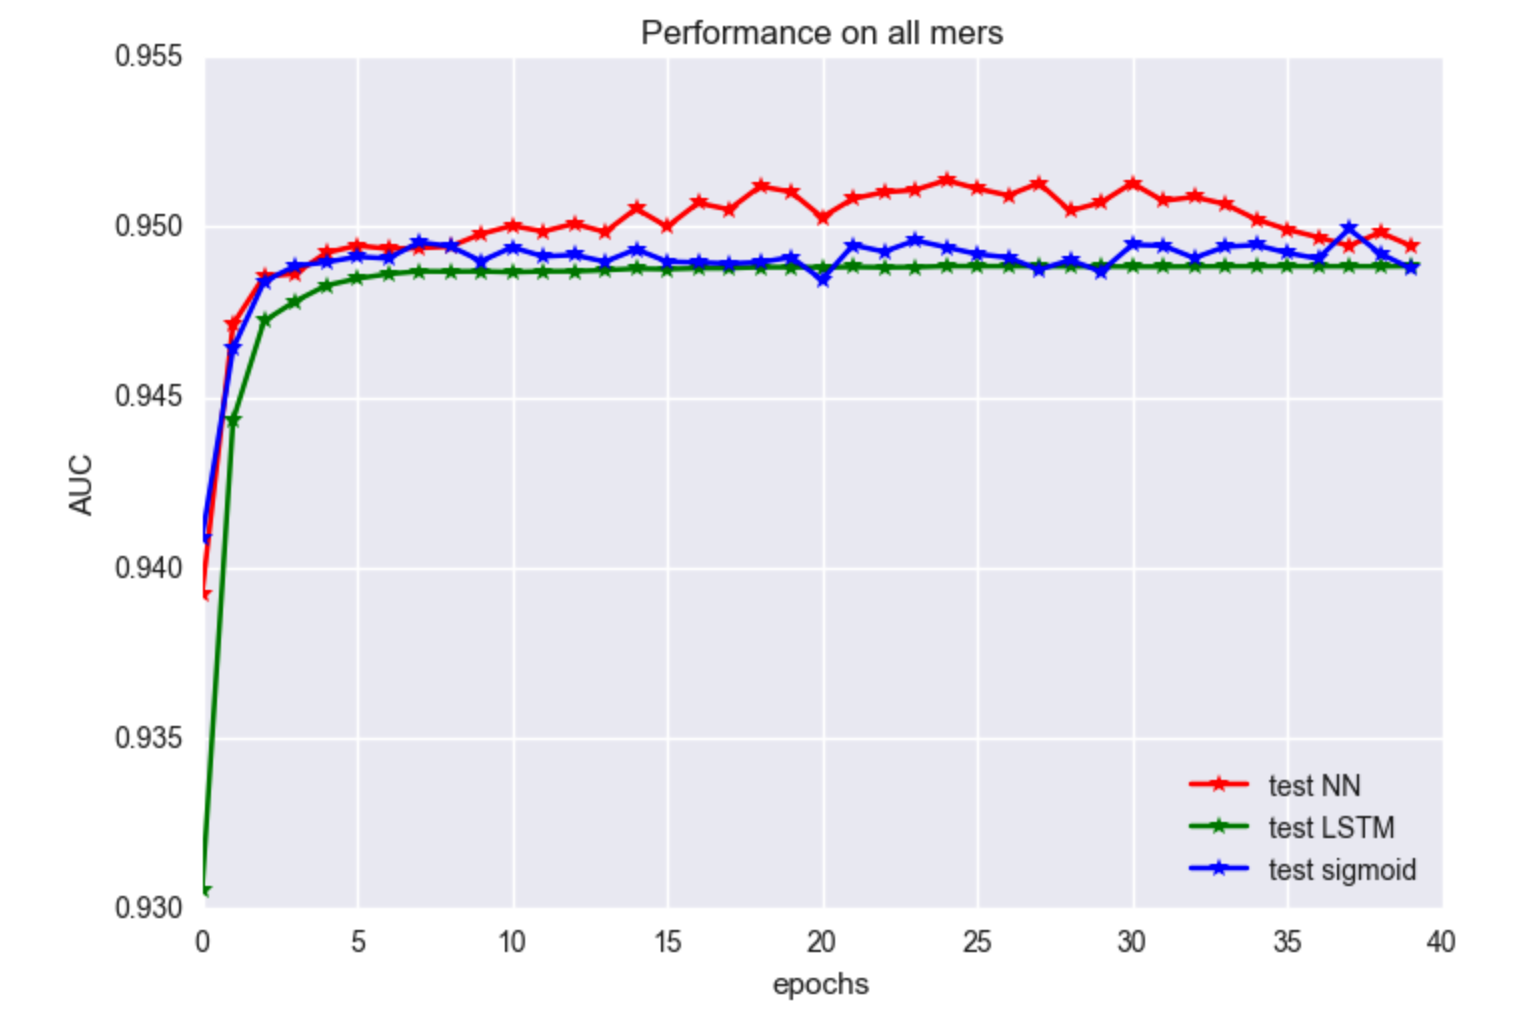
\includegraphics[scale = 0.3]{LSTM_vs_FFN_vs_sigmoid.png}

Segmenting the test set into 9 mers and non 9 mers, one notices that LSTMs worse performance stems from its worse performance on non 9 mers, while FFNN and LSTM perform about the same on 9 mers.\\

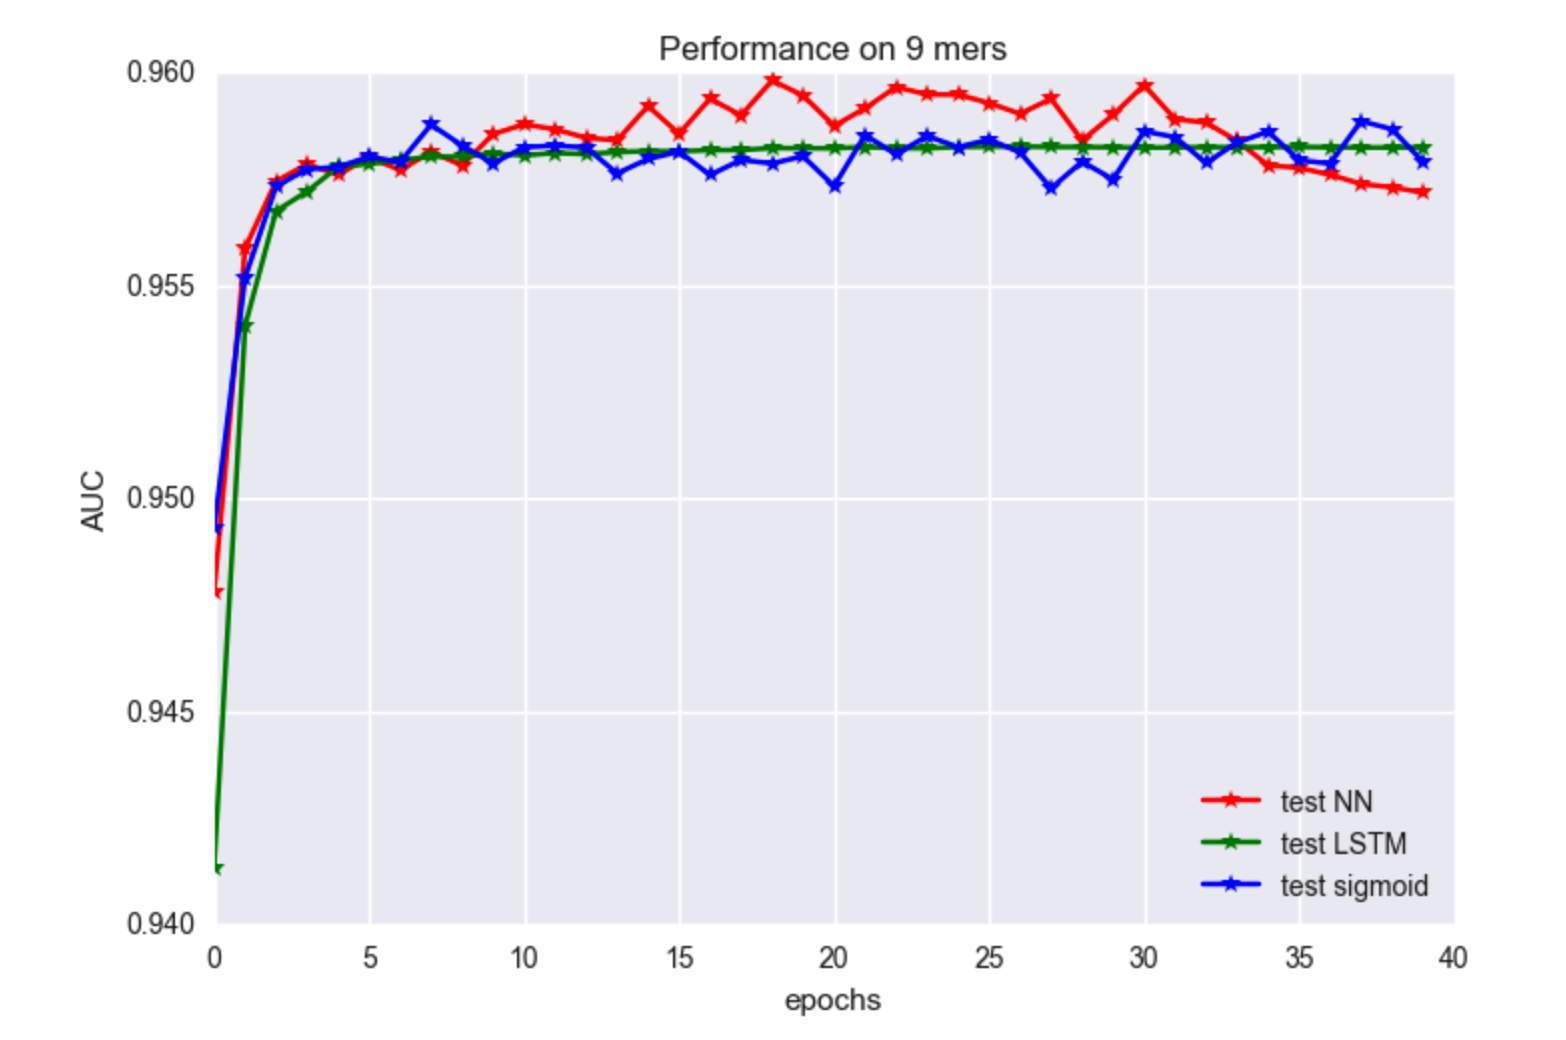
\includegraphics[scale = 0.3]{LSTM_vs_FFN_vs_sigmoid_9mers.png}
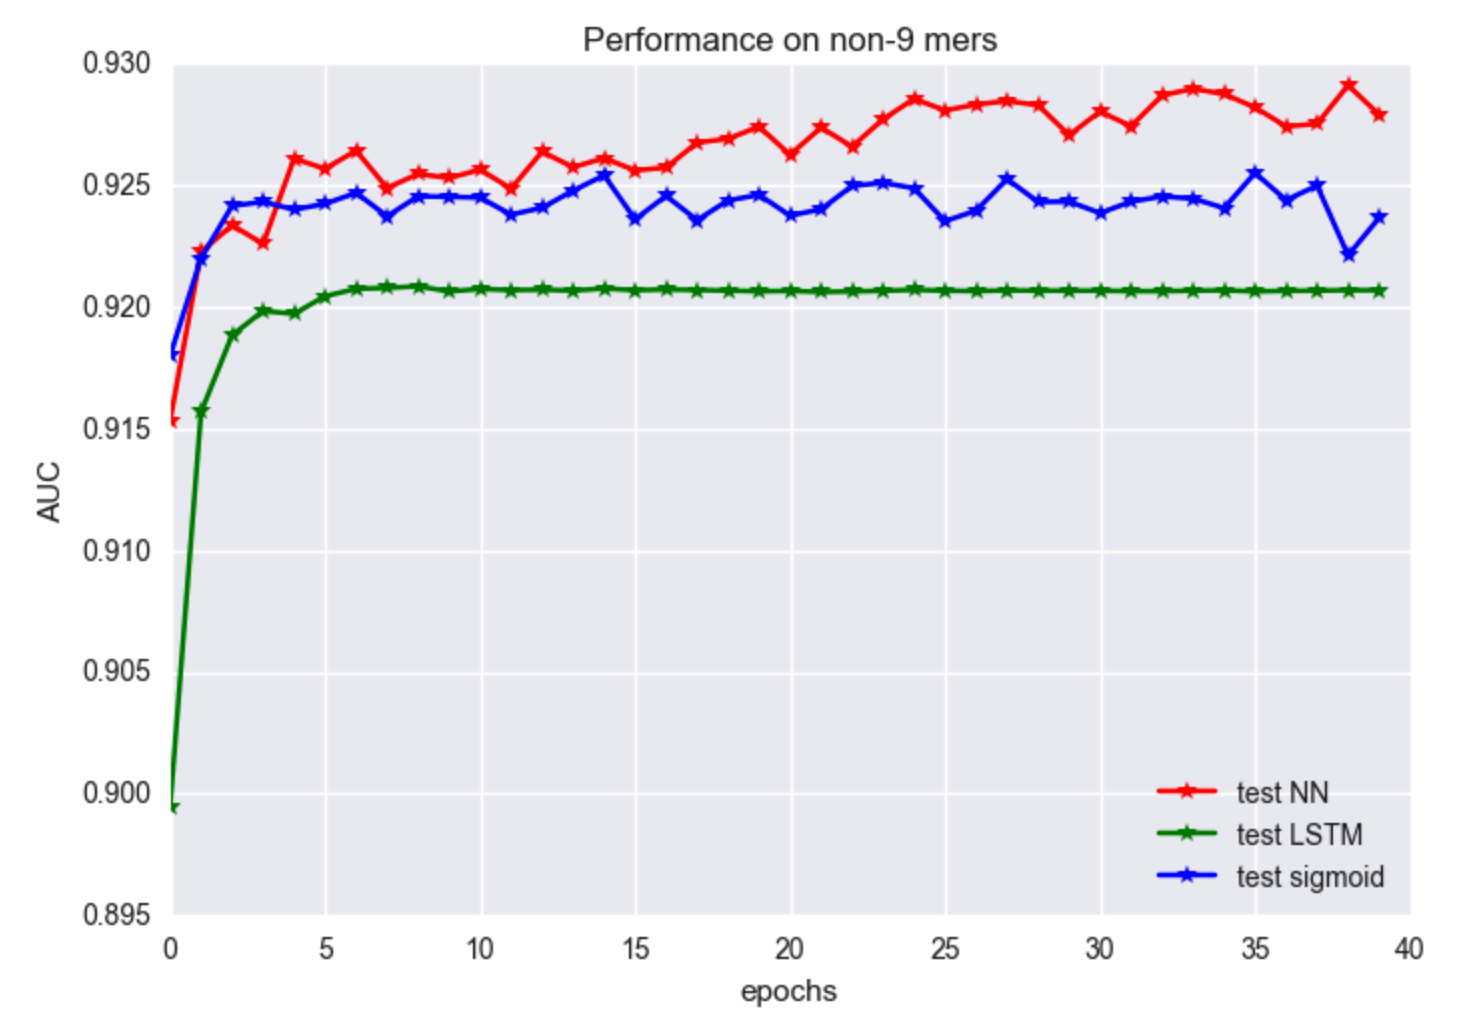
\includegraphics[scale = 0.3]{LSTM_vs_FFN_vs_sigmoid_non9mers.png}

Quite surprisingly a simple sigmoid layer does a better job on non 9 mers than LSTM. This either means that kmer-index-encoding is doing particularly well, or LSTM is doing particularly bad. (If we are able to get the LSTM to mimick the kmer index encoding` we have a good chance of improving performance on non 9 mers. )

%=========================================================
\section{Hints for improvement}
%=========================================================

\subsection{kmer-index-encoded LSTM}

In this subsection, we have trained and tested LSTM endowed with kmer-index-encoding in order to see whether the overall performance improves compared to a simple LSTM and if so, whether the improvement is most visible on 9 mers or non-9 mers. 

\subsubsection{performance on all mers}

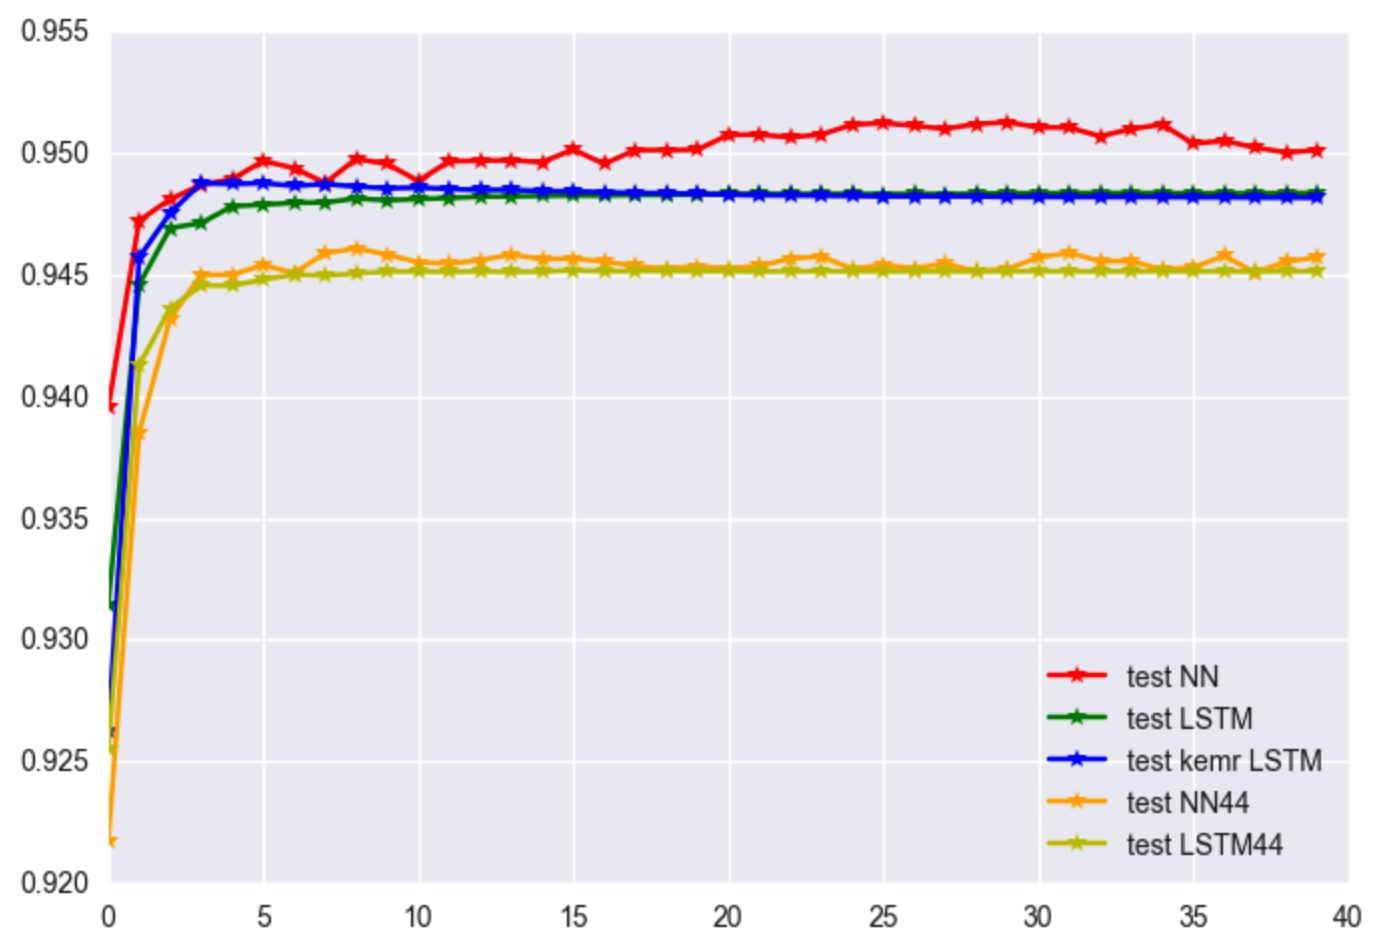
\includegraphics[scale = 0.3]{kmerLSTM_allmers.png}

\subsubsection{performance on 9 mers}

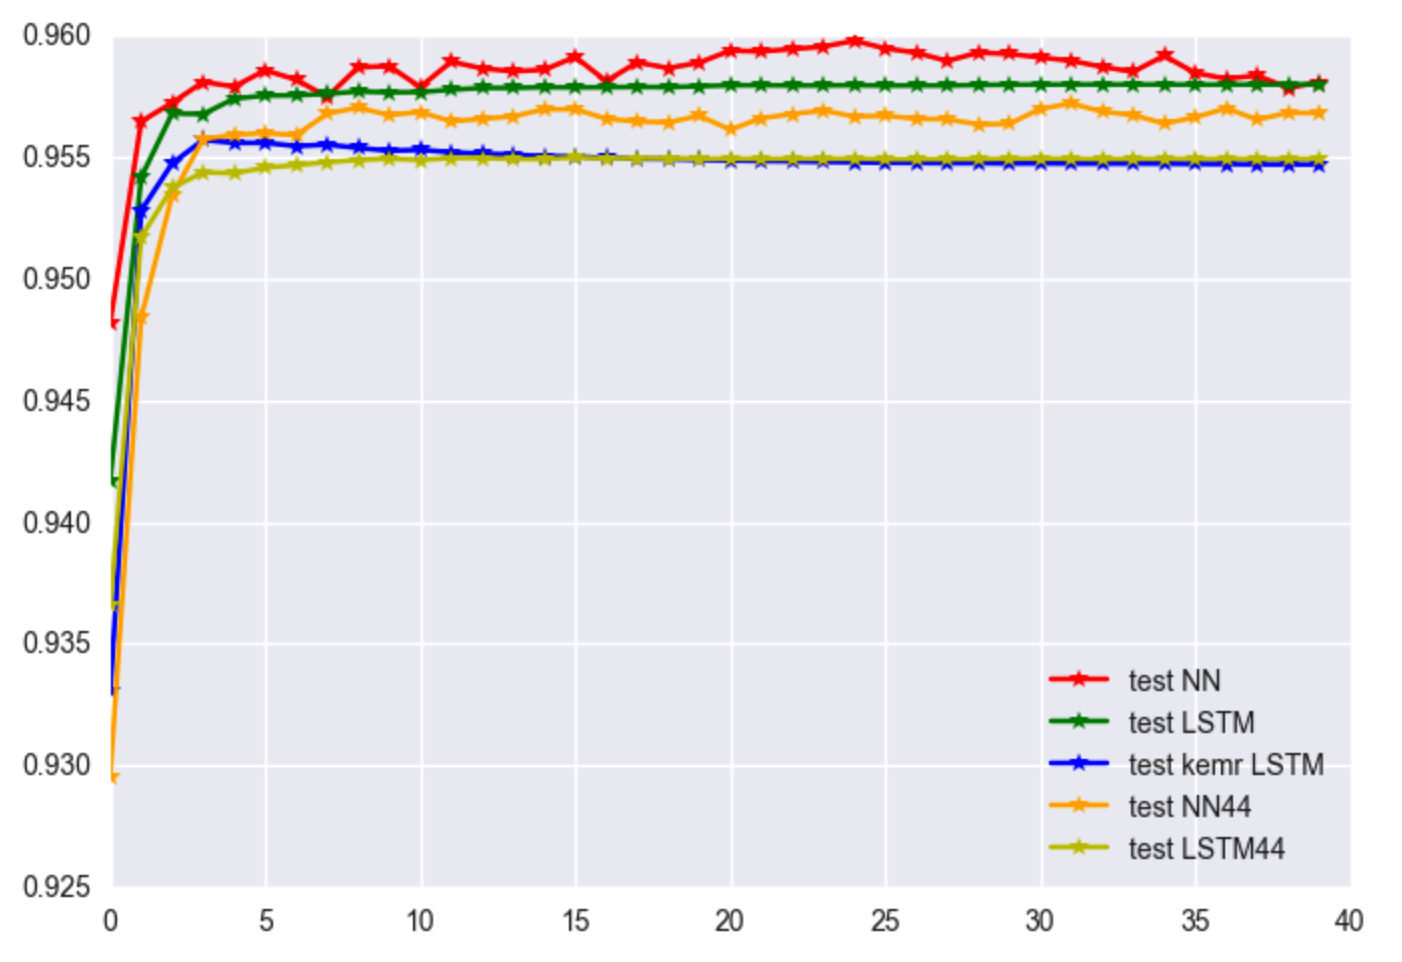
\includegraphics[scale = 0.3]{kmerLSTM_9mers.png}

\subsubsection{performance on non 9 mers}

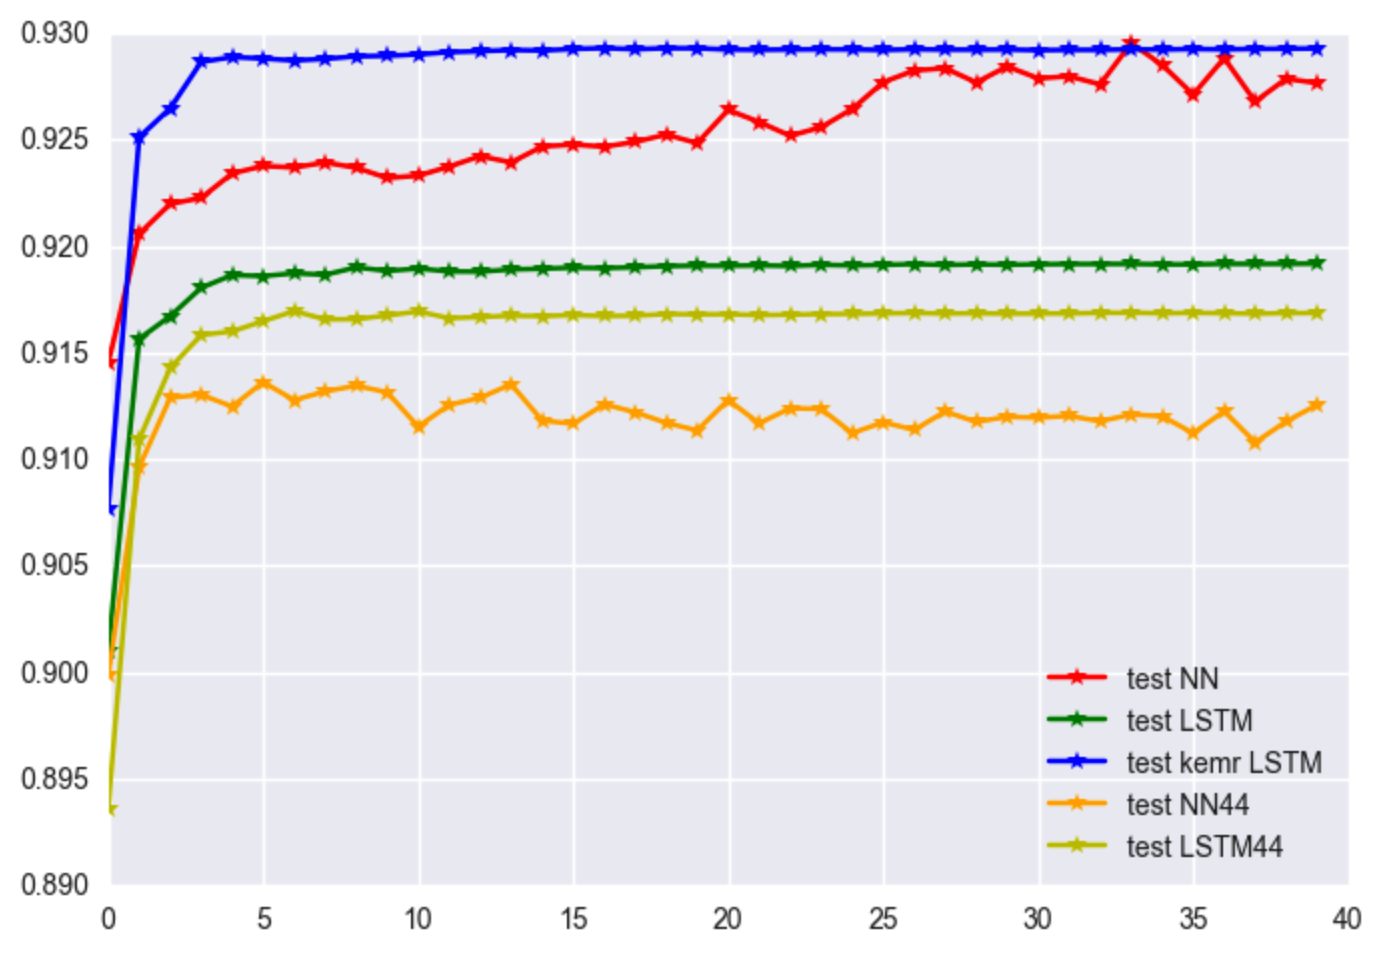
\includegraphics[scale = 0.3]{kmerLSTM_non9mers.png}

we clearly see an improvement of the kmer LSTM on the non 9 mers. 

(image)

%=========================================================
\begin{small}
\setlength{\bibsep}{0.03cm}
%\bibliographystyle{abbrv}
\bibliographystyle{ieeetr}
%\bibliographystyle{apa}
\bibliography{refs}
\end{small}
%=========================================================




\end{document}

\grid
